\documentclass[12pt]{article}
\usepackage[english]{babel}
\usepackage[letterpaper,top=2cm,bottom=2cm,left=3cm,right=3cm,marginparwidth=1.75cm]{geometry}
\usepackage{amsmath}
\usepackage{graphicx}
\usepackage{gensymb}
\title{STAT-UB 103 Homework 2}
\author{Ishan Pranav}
\date{February 2, 2023}
\renewcommand{\thesubsection}{\thesection.\alph{subsection}}
\renewcommand{\theenumi}{\alph{enumi}}
\newcommand{\degreef}{\degree F}
\begin{document}
\maketitle
\section{Data on body temperatures}
\begin{enumerate}
\item The data do seem to have a reasonably bell-shaped distribution. There are no obvious outliers. 

\item I think that the population mean for body temperatures is 98.6\degreef since that is the number that I have been hearing since I was very young. 

\item
Based on the histogram in Figure~\ref{fig:temperaturehistogram}, the sample mean does seem reasonably close to the “known” population mean. From the histogram, the sample mean seems to be around 98.3\degreef, which is reasonably close to our “known” value of 98.6\degreef. 

\begin{figure}
\begin{center}
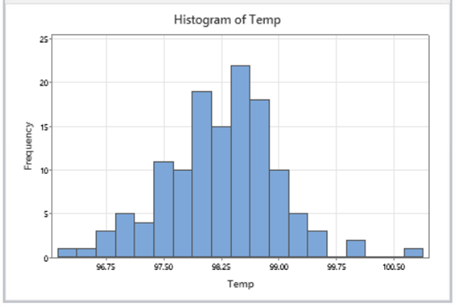
\includegraphics[width=4in]{images/temperature-histogram.png}
\end{center}
\caption{Histogram of body temperature.\label{fig:temperaturehistogram}}
\end{figure}

\item Based on descriptive statistics, the sample mean is 98.249\degreef. This is reasonably close to our “known” value of 98.6\degreef. 

\item
The median is greater than the mean by only 0.051\degreef. This indicates that the data are roughly symmetrical but slightly left skewed.

\begin{itemize}
    \item Median: 98.3\degreef
    \item Range: 4.5\degreef
    \item Interquartile range: 0.9\degreef
\end{itemize}
\end{enumerate}

\section{Data on the stock returns and earnings per share}
\begin{figure}
\begin{center}
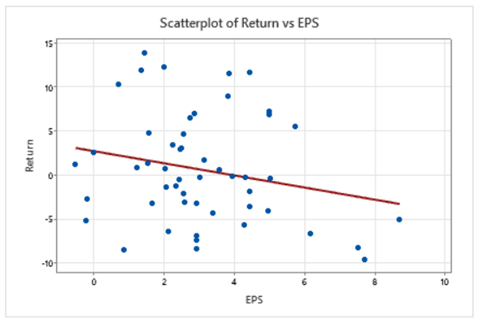
\includegraphics[width=4in]{images/return-eps-scatterplot.png}
\end{center}
\caption{Scatterplot of return and earnings per share.\label{fig:returnepsscatterplot}}
\end{figure}
Yes, the scatterplot in Figure~\ref{fig:returnepsscatterplot} suggests a weak negative relationship between stock returns and earnings per share. I would have expected a stronger positive correlation between the two variables. The company with the highest value of earnings per share was the General Motors Corporation. No, the return for this company was quite negative. 

\section{Data on monthly private residential construction expenditures}
\begin{figure}
\begin{center}
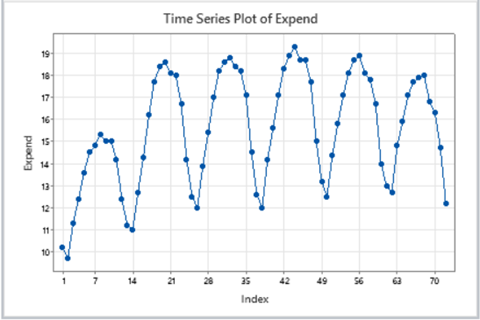
\includegraphics[width=4in]{images/expenditures-time-series.png}
\end{center}
\caption{Time series of expenditures.}
\end{figure}
There is seasonality in the data since some months every year have higher expenditures than others. The overall trend sees expenditures tend to be increasing for the first three years and then decreasing for the next three years. The first year, 1988, is exceptionally low and can likely be explained by the business cycle. Perhaps there was a poor construction economy in 1988. 

Expenditures reach a peak or a trough every sixth or seventh month. This is expected because it is likely that construction occurs during seasons of good weather like spring and peaks in the summer. Similarly, construction falls after the summer as autumn approaches winter. Inclement weather likely hinders construction. If I had to predict monthly private residential construction expenditures for July 1994, I would estimate around 17.8. Peak expenditures have been falling since 1991, so it is unlikely that July 1994 would exceed the peak reached in July 1993, which is 18. This is why 17.8 or 17.9 are reasonable estimates. 

\section{Data on the number of copies made on a self-service copying machine at a copy center}
\begin{figure}
\begin{center}
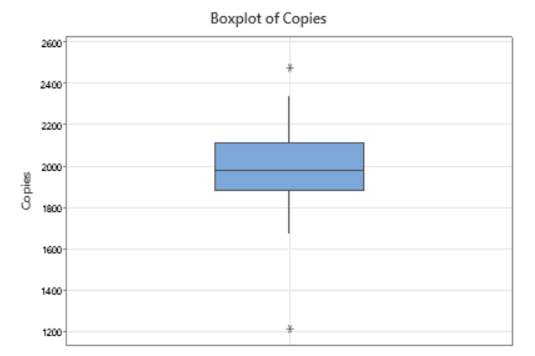
\includegraphics[width=4in]{images/copies-boxplot.png}
\end{center}
\caption{Boxplot of copies. There are two outliers: 2477 copies made on day 5 and 1207 copies made on day 25.\label{fig:copiesboxplot}}
\end{figure}
\begin{enumerate}
\item See Figure~\ref{fig:copiesboxplot}.
\item
\begin{itemize}
    \item Mean: 1985.5 copies
    \item Standard deviation: 200.8 copies
\end{itemize}
\item
\begin{itemize}
    \item Mean: 1992.3 copies
    \item Standard deviation: 146.9
\end{itemize}
The standard deviation has changed more because the variation in the data has been reduced by the elimination of outliers.
\item Outliers have a greater impact on the standard deviation than on the mean because the standard deviation is a measure of variation. The elimination of outliers reduces the variation. Because we are removing a high outlier and a low outlier, the mean is relatively unchanged since they offset one another.
\end{enumerate}
\section{Daily returns on the Dow Jones Industrial Average}
\begin{figure}
\begin{center}
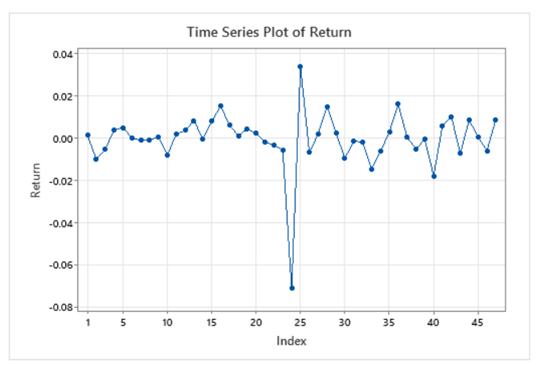
\includegraphics[width=4in]{images/return-time-series.png}
\end{center}
\caption{Time series of returns.\label{fig:returntimeseries}}
\end{figure}
\begin{figure}
\begin{center}
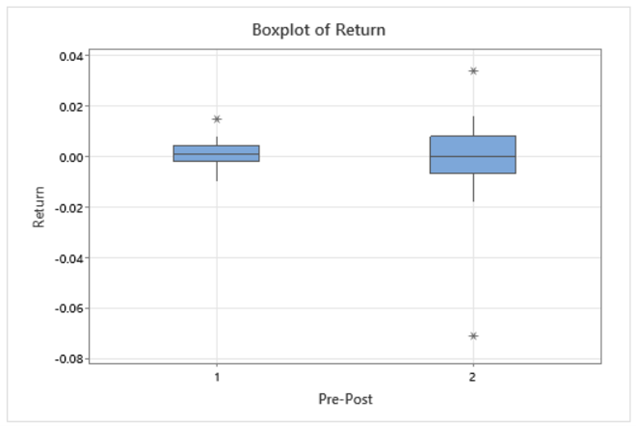
\includegraphics[width=4in]{images/return-boxplot.png}
\end{center}
\caption{Boxplot of return.}
\end{figure}
\begin{enumerate}
    \item There isn't visible seasonality in the data since peaks and troughs are not consistent. The overall trend is constant. The exceptional activity on day 24 is an example of a business-cycle fluctuation. One possible forecast is that the market will remain constant but remain vulnerable to arbitrary fluctuations in the business cycle.
    \item In this case, the population will be the 47 observations. The population mean is approximately 0.0006 and the population standard deviation is approximately 0.0137. The 24\textsuperscript{th} observation is approximately 0.0716 (which represents a roughly 7.15 percent drop in the market). The standardized $z$ score is approximately -5.189, meaning that the 24\textsuperscript{th} observation was more than 5 standard deviations below the mean.
    \item The 25\textsuperscript{th} observation is approximately 0.0337 (a 3.37 percent increase in the market). The standardized $z$ score is approximately 2.507, meaning that the next day's change was more than 2.5 standard deviations above the mean.
    \item After a crash, the volatility of returns increases. This is illustrated on the time series plot in Figure~\ref{fig:returntimeseries}, where the distances between peaks and troughs are higher after the crash compared to before the crash.
\end{enumerate}
\section{Data on the 1970 draft lottery}
\begin{figure}
\begin{center}
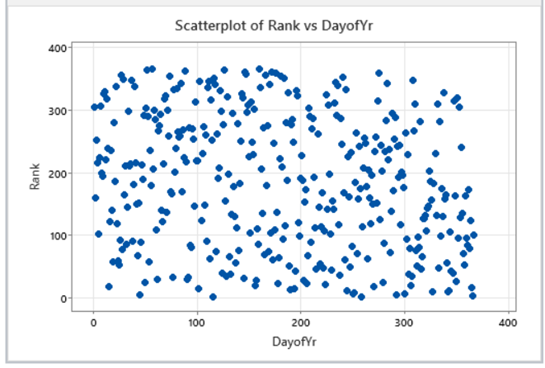
\includegraphics[width=4in]{images/rank-day-scatterplot.png}
\end{center}
\caption{Scatterplot of rank and day of the year.\label{fig:rankdayscatterplot}}
\end{figure}
\begin{figure}
\begin{center}
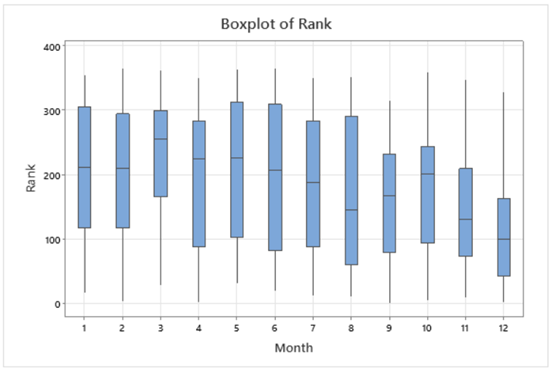
\includegraphics[width=4in]{images/rank-boxplot.png}
\end{center}
\caption{Boxplot of rank.}
\end{figure}
\begin{enumerate}
    \item The scatterplot in Figure~\ref{fig:rankdayscatterplot} does not show any obvious patterns.
    \item The decreasing medians indicate that later months tend to have lower ranks and are more likely to be chosen before others. The month of December seems to be systemically receiving the lowest rankings. The procedure for the lottery is not fair: the median rank in December was about 100, while in January the median rank was over 200. Since months were stacked onto the vat in order (last in, first out), the December dates were on the top and would remain there if the vat was not mixed thoroughly. It is likely that “a few minutes” was not enough to evenly mix the dates in the pool. 
\end{enumerate}
\end{document}
